\documentclass[convert={convertexe={magick.exe},density=150,outext=.png}]{standalone}
\usepackage{tikz}
\usetikzlibrary{decorations,decorations.markings,decorations.text}
\usepackage{xcolor}
\definecolor{PCB1}{RGB}{132,223,132}
\definecolor{PCB2}{RGB}{150,250,110}
\definecolor{Trace}{RGB}{255,203,0}

\begin{document}
 \pgfkeys{/pgf/decoration/.cd,
      distance/.initial=10pt
}  

\pgfdeclaredecoration{add dim}{final}{
\state{final}{% 
\pgfmathsetmacro{\dist}{5pt*\pgfkeysvalueof{/pgf/decoration/distance}/abs(\pgfkeysvalueof{/pgf/decoration/distance})} 
          \pgfpathmoveto{\pgfpoint{0pt}{0pt}}             
          \pgfpathlineto{\pgfpoint{0pt}{2*\dist}}   
          \pgfpathmoveto{\pgfpoint{\pgfdecoratedpathlength}{0pt}} 
          \pgfpathlineto{\pgfpoint{\pgfdecoratedpathlength}{2*\dist}}
           \pgfusepath{stroke} 
%          \pgfsetdash{{0.1cm}{0.1cm}{0.1cm}{0.1cm}}{0cm}     
          \pgfsetarrowsstart{latex}
          \pgfsetarrowsend{latex}  
          \pgfpathmoveto{\pgfpoint{0pt}{\dist}}
          \pgfpathlineto{\pgfpoint{\pgfdecoratedpathlength}{\dist}} 
          \pgfusepath{stroke} 
          \pgfsetdash{}{0pt}
          \pgfpathmoveto{\pgfpoint{0pt}{0pt}}
          \pgfpathlineto{\pgfpoint{\pgfdecoratedpathlength}{0pt}}
          \pgfusepath{stroke}
}}

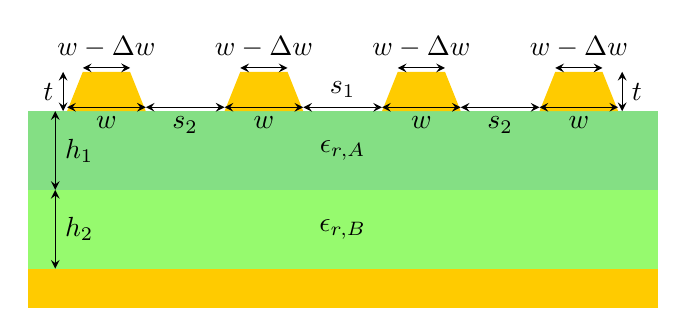
\begin{tikzpicture}[>=stealth]
\fill[PCB1] (-4,-1) rectangle (4,0);
\fill[PCB2] (-4,-2) rectangle (4,-1);
\fill[Trace] (-1.5,0) -- (-0.5,0) -- (-0.7,0.5) -- (-1.3,0.5) -- cycle;
\fill[Trace] (0.5,0) -- (1.5,0) -- (1.3,0.5) -- (0.7,0.5) -- cycle;
\fill[Trace] (-3.5,0) -- (-2.5,0) -- (-2.7,0.5) -- (-3.3,0.5) -- cycle;
\fill[Trace] (2.5,0) -- (3.5,0) -- (3.3,0.5) -- (2.7,0.5) -- cycle;
\fill[Trace] (-4,-2.5) rectangle (4,-2);

\draw[<->] (-1.3,0.55) -- (-0.7,0.55) node[midway, above] {$w - \Delta w$};
\draw[<->] (0.7,0.55) -- (1.3,0.55) node[midway, above] {$w - \Delta w$};
\draw[<->] (0.5,0.05) -- (1.5,0.05) node[midway, below] {$w$};
\draw[<->] (-1.5,0.05) -- (-0.5,0.05) node[midway, below] {$w$};
\draw[<->] (-3.3,0.55) -- (-2.7,0.55) node[midway, above] {$w - \Delta w$};
\draw[<->] (2.7,0.55) -- (3.3,0.55) node[midway, above] {$w - \Delta w$};
\draw[<->] (2.5,0.05) -- (3.5,0.05) node[midway, below] {$w$};
\draw[<->] (-3.5,0.05) -- (-2.5,0.05) node[midway, below] {$w$};
\draw[<->] (-0.5,0.05) -- (0.5,0.05) node[midway, above] {$s_1$};
\draw[<->] (-2.5,0.05) -- (-1.5,0.05) node[midway, below] {$s_2$};
\draw[<->] (1.5,0.05) -- (2.5,0.05) node[midway, below] {$s_2$};
\draw[<->] (-3.55,0) -- (-3.55,0.5) node[midway, left] {$t$};
\draw[<->] (3.55,0) -- (3.55,0.5) node[midway, right] {$t$};
\draw[<->] (-3.65,-1.0) -- (-3.65,0) node[midway, right] {$h_1$};
\draw[<->] (-3.65,-2.0) -- (-3.65,-1.0) node[midway, right] {$h_2$};

\node at (0,-0.5) {$\epsilon_{r,A}$};
\node at (0,-1.5) {$\epsilon_{r,B}$};
\end{tikzpicture}

\end{document}